\documentclass[tikz,border=2pt]{standalone}
\usepackage{amsmath}
\usepackage{pgfplots}
\pgfplotsset{compat=1.18}

\begin{document}
% Normal convergence looks only at the sizes ||f_n||_oo of the terms: here ||f_n||_oo = 1/n^2,
% whose partial sums S_N climb to pi^2/6, so the series of functions converges normally.
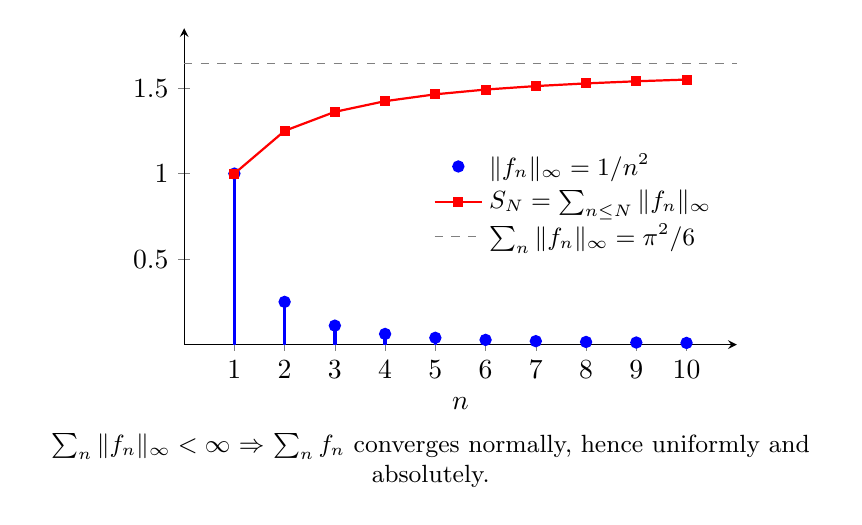
\begin{tikzpicture}
	\begin{axis}[
		axis lines=left,
		xmin=0, xmax=11, ymin=0, ymax=1.85,
		xtick={1,...,10}, ytick={0.5,1,1.5},
		xlabel={$n$},
		width=8.6cm, height=5.6cm, clip=false,
		legend style={draw=none, fill=none, font=\small, at={(0.98,0.64)}, anchor=north east}, legend cell align=left
		]
		\addplot[ycomb, blue, very thick, mark=*, mark size=1.6pt] coordinates {(1,1) (2,0.25) (3,0.1111) (4,0.0625) (5,0.04) (6,0.0278) (7,0.0204) (8,0.0156) (9,0.0123) (10,0.01)};
		\addlegendentry{$\|f_n\|_\infty=1/n^2$}
		\addplot[red, thick, mark=square*, mark size=1.4pt] coordinates {(1,1) (2,1.25) (3,1.3611) (4,1.4236) (5,1.4636) (6,1.4914) (7,1.5118) (8,1.5274) (9,1.5398) (10,1.5498)};
		\addlegendentry{$S_N=\sum_{n\le N}\|f_n\|_\infty$}
		\addplot[gray, dashed, domain=0:11, samples=2] {1.6449};
		\addlegendentry{$\sum_n\|f_n\|_\infty=\pi^2/6$}
	\end{axis}
	\node[anchor=north, align=flush center, text width=10cm, font=\small] at ([yshift=-2pt]current axis.outer south) {$\sum_n\|f_n\|_\infty<\infty$ $\Rightarrow$ $\sum_n f_n$ converges normally, hence uniformly and absolutely.};
\end{tikzpicture}
\end{document}
